\section{Avaliação dos Resultados}

%Nesta seção, os resultados são apresentados em gráficos. Para cada figura,
%importante lembrar que deve ter texto com explicação.
%Caso a metodologia de avaliação não tenha sido descrita em uma seção específica,
%esta pode ser descrita no início desta seção.

Nos gráficos subsequentes, há uma demonstração de como a memória cache se comporta 
ao ser usada com um grande conjunto de instruções de \emph{load} e \emph{store} 
(maior que sua capacidade) em cenários com caches de 2, 4, 8 e 16 linhas.
Para fazer esses testes utilizamos um conjunto de 10, 50, 100, 250, 500, 750, 1.000 e 10.000 
instruções.

\subsection{Gráficos de hit rate por número de instruções}

  \begin{figure}[H]

    \centering
    
  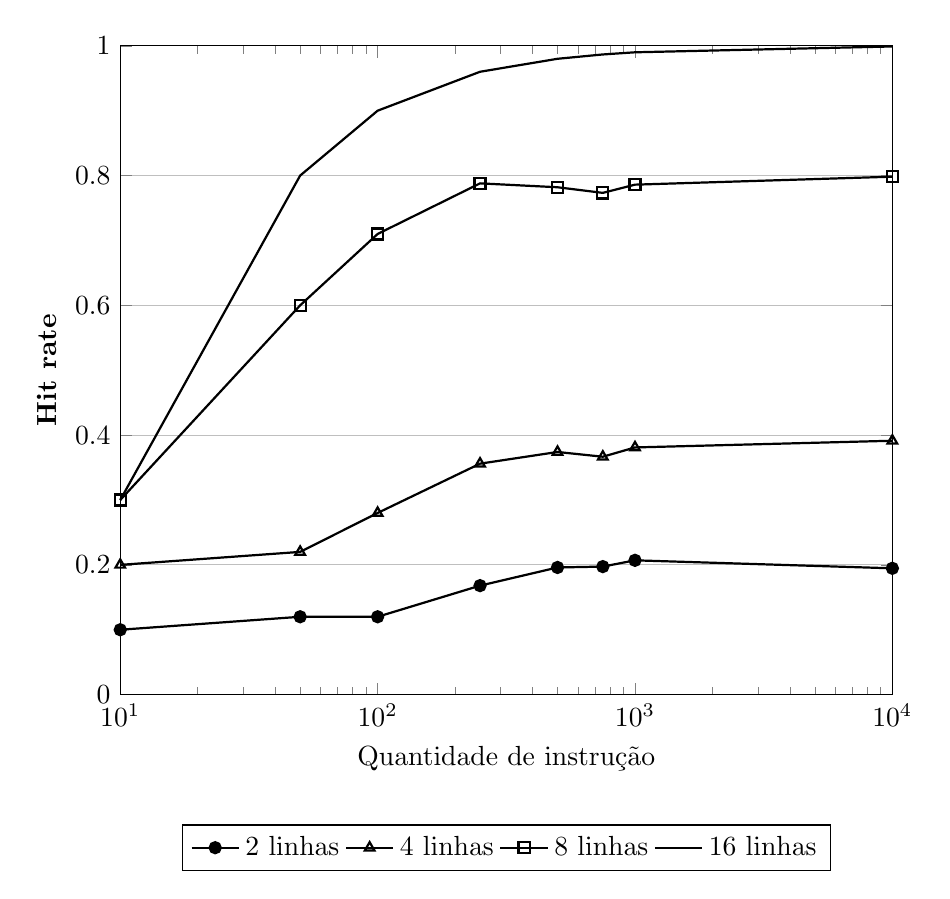
\begin{tikzpicture}

    \begin{axis}[
      width =\linewidth - 21,
      xlabel=Quantidade de instrução,
      ylabel=\textbf{Hit rate},
      domain = 1:10000,
      xmin=10, xmax=10000,
      ymin=0, ymax=1,
      xmode = log,
      log basis x={10},
      clip=false,
      every axis plot/.append style={thick},
      ymajorgrids=true,
      legend  style={at={(0.5 ,-0.20)},
      anchor=north,legend  columns =-1},
    ]
    \addplot [mark=*] coordinates {
      (10, 0.1)
      (50, 0.12)
      (100, 0.12)
      (250, 0.168)
      (500, 0.196)
      (750, 0.19733334)
      (1000, 0.207)
      (10000, 0.1947)
    };
    \addplot [mark=triangle] coordinates {
      (10, 0.2)
      (50, 0.22)
      (100, 0.28)
      (250, 0.356)
      (500, 0.374)
      (750, 0.36666667)
      (1000, 0.381)
      (10000, 0.3913)
  };
  \addplot [mark=square] coordinates {
      (10, 0.3)
      (50, 0.6)
      (100, 0.71)
      (250, 0.788)
      (500, 0.782)
      (750, 0.7733333)
      (1000, 0.786)
      (10000, 0.7983)
  };
  \addplot [solid] coordinates {
      (10, 0.3)
      (50, 0.8)
      (100, 0.9)
      (250, 0.96)
      (500, 0.98)
      (750, 0.9866667)
      (1000, 0.99)
      (10000, 0.999)
  };

  \legend{2 linhas, 4 linhas, 8 linhas, 16 linhas}

    \end{axis}

  \end{tikzpicture}
  \caption{\textit{\textbf{Cache com algoritmo de substituição FIFO}}}
  \label{ima1}
\end{figure}

  \begin{figure}[H]
  
  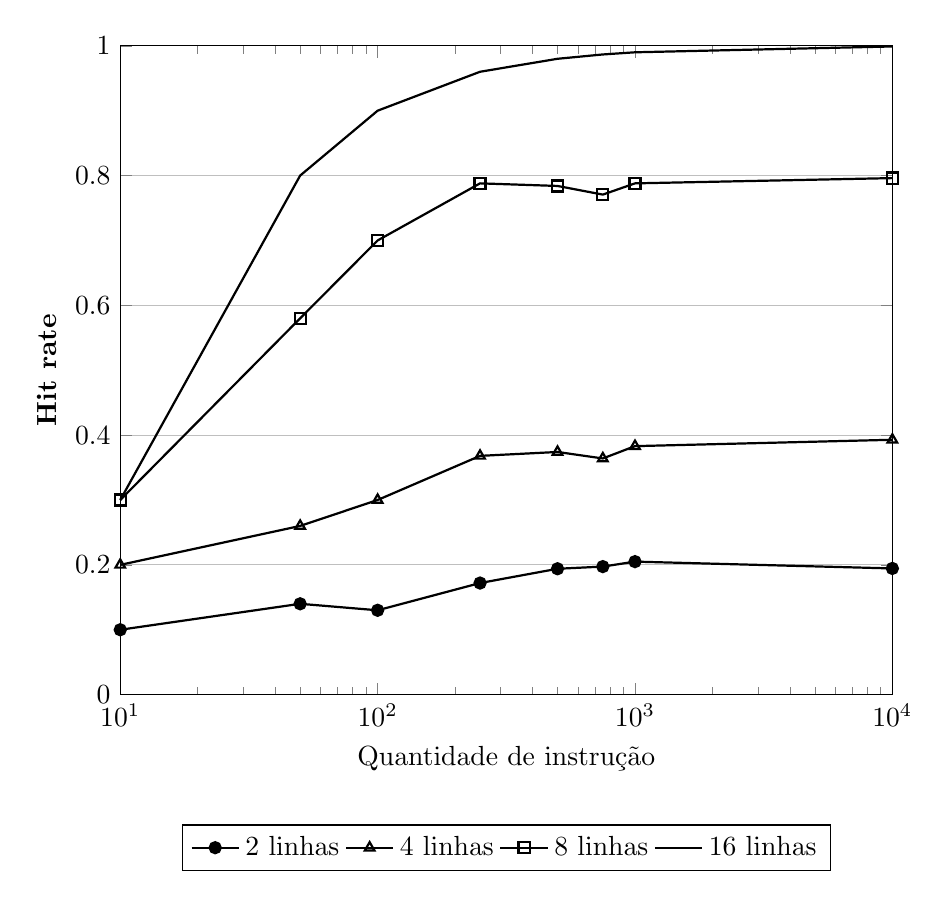
\begin{tikzpicture}
    
    \begin{axis}[
      width =\linewidth - 21,
      xlabel=Quantidade de instrução,
      ylabel=\textbf{Hit rate},
      domain = 1:10000,
      xmin=10, xmax=10000,
      ymin=0, ymax=1,
      xmode = log,
      log basis x={10},
      clip=false,
      every axis plot/.append style={thick},
      ymajorgrids=true,
      legend  style={at={(0.5 ,-0.20)},
      anchor=north,legend  columns =-1},
    ]
    \addplot [mark=*] coordinates {
      (10, 0.1)
      (50, 0.14)
      (100, 0.13)
      (250, 0.172)
      (500, 0.194)
      (750, 0.19733334)
      (1000, 0.205)
      (10000, 0.1945)
    };
    \addplot [mark=triangle] coordinates {
      (10, 0.2)
      (50, 0.26)
      (100, 0.3)
      (250, 0.368)
      (500, 0.374)
      (750, 0.364)
      (1000, 0.383)
      (10000, 0.3928)
  };
  \addplot [mark=square] coordinates {
      (10, 0.3)
      (50, 0.58)
      (100, 0.7)
      (250, 0.788)
      (500, 0.784)
      (750, 0.77066666)
      (1000, 0.788)
      (10000, 0.7961)
  };
  \addplot [solid] coordinates {
      (10, 0.3)
      (50, 0.8)
      (100, 0.9)
      (250, 0.96)
      (500, 0.98)
      (750, 0.9866667)
      (1000, 0.99)
      (10000, 0.999)
  };

  \legend{2 linhas, 4 linhas, 8 linhas, 16 linhas}

    \end{axis}
    
  \end{tikzpicture}

  \caption{\textit{\textbf{Cache com algoritmo de substituição LRU}}}
  \label{ima2}
\end{figure}

Os dois gráficos mostrados foram montados usando os valores que extraímos. Nota-se que os resultados foram muito próximos, aos resultados de James E. Smith
e James R. Goodman\cite{b1}. Considerando que no início, pensávamos que haveria uma diferença significativa entre os algoritmos LRU e FIFO para substituição
de valores na cache, achamos que nossos testes estavam errados e que precisaríamos refazê-los, ao ler o artigo vimos que os nossos resultados na verdade estavam
bem dentro do esperado.
  
Nossos testes apenas foram feitos usando caches completamente associativos, pensamos em fazer com a associatividade por conjunto e direta, mas depois de resultados
tão inesperados, pensamos em pesquisar outros artigos relacionados que já tivessem feito esses testes para comparar os resultados e ver se os resultados seriam
diferentes. Ao ver os dados do artigo\cite{b1}, descobrimos que teríamos valores bem semelhantes dentro dessas três arquiteturas. 

Para colocar em perspectiva nossos resultados, os dados em \cite{b2} foram
medidos usando benchmark mantido pelos grupos de pesquisa, considerando uma
cache de 2KB com 32 bytes de linhas. Eles são expressos em termos da porcentagem de
hits na cache detectada pela análise feita pelo grupo. A política de LRU se demonstrou
mais eficiente do que a PLRU e a política aleatória de troca, em apenas alguns casos que
não houve diferença entre as análises, porém na pesquisa d \cite{b2} foi utilizado também
como parâmetro o tempo de vida mínimo de um elemento na cache(\emph{Minimum life span)})


\subsection{Tempo total de acesso aos dados por quantidade de instruções}

\raggedbottom

\begin{figure}[H]

  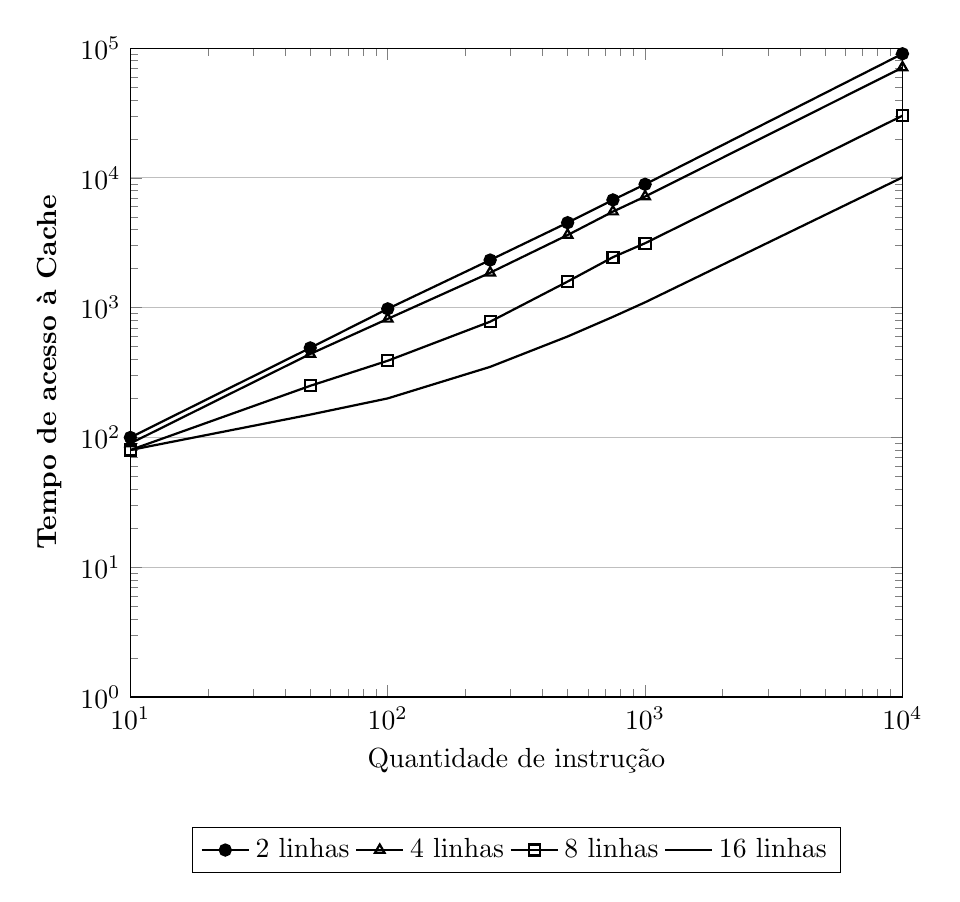
\begin{tikzpicture}

    \begin{axis}[
      width =\linewidth - 21,
      xlabel=Quantidade de instrução,
      ylabel=\textbf{Tempo de acesso à Cache},
      domain = 1:10000,
      xmin=10, xmax=10000,
      ymin=1, ymax=100000,
      ymode = log,
      log basis y={10},
      xmode = log,
      log basis x={10},
      clip=false,
      every axis plot/.append style={thick},
      ymajorgrids=true,
      legend  style={at={(0.5 ,-0.20)},
      anchor=north,legend  columns =-1},
    ]
    \addplot [mark=*] coordinates {
      (10, 100)
      (50, 490)
      (100, 980)
      (250, 2330)
      (500, 4520)
      (750, 6770)
      (1000, 8930)
      (10000, 90530)
    };
    \addplot [mark=triangle] coordinates {
      (10, 90)
      (50, 440)
      (100, 820)
      (250, 1860)
      (500, 3630)
      (750, 5500)
      (1000, 7190)
      (10000, 70870)
  };
  \addplot [mark=square] coordinates {
      (10, 80)
      (50, 250)
      (100, 390)
      (250, 780)
      (500, 1590)
      (750, 2450)
      (1000, 3140)
      (10000, 30170)
  };
  \addplot [solid] coordinates {
      (10, 80)
      (50, 150)
      (100, 200)
      (250, 350)
      (500, 600)
      (750, 850)
      (1000, 1100)
      (10000, 10100)
  };

  \legend{2 linhas, 4 linhas, 8 linhas, 16 linhas}

    \end{axis}
    
  \end{tikzpicture}
  \caption{\textit{\textbf{Tempo total de acesso aos dados com algoritmo FIFO}}}
  \label{ima3}
\end{figure}

  \begin{figure}[H]

  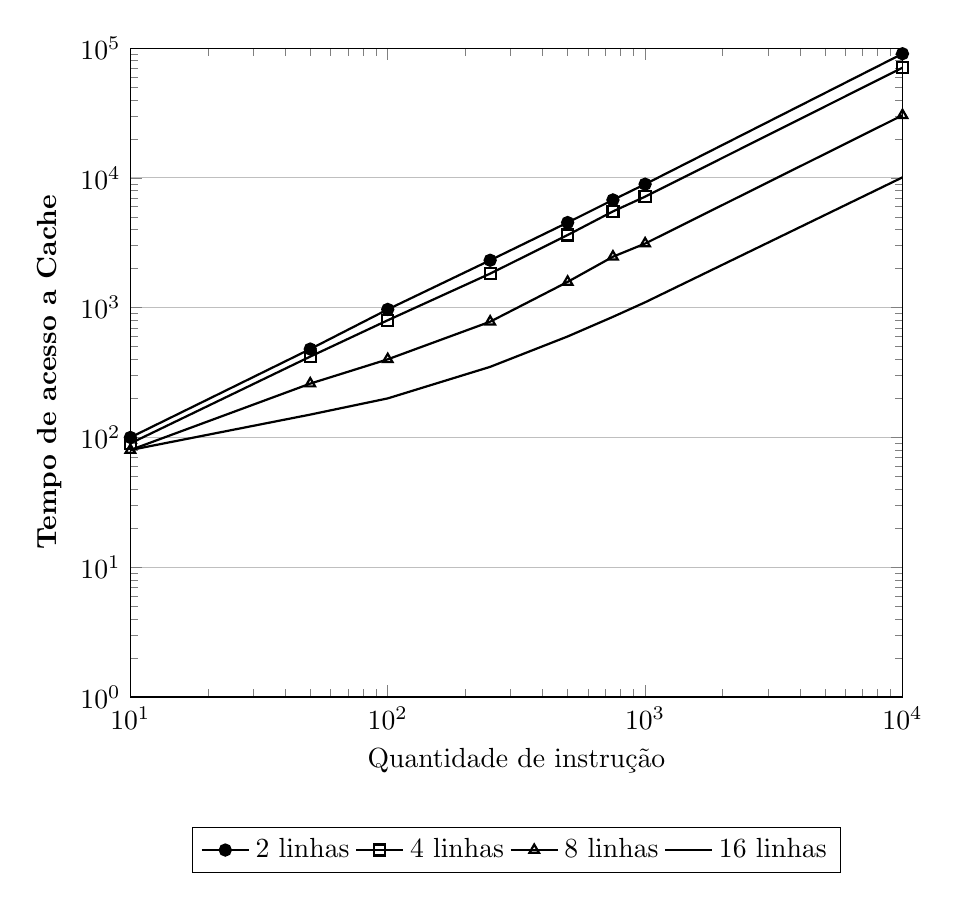
\begin{tikzpicture}

    \begin{axis}[
      width =\linewidth - 21,
      xlabel=Quantidade de instrução,
      ylabel=\textbf{Tempo de acesso a Cache},
      domain = 1:10000,
      xmin=10, xmax=10000,
      ymin=1, ymax=100000,
      ymode = log,
      log basis y={10},
      xmode = log,
      log basis x={10},
      clip=false,
      every axis plot/.append style={thick},
      ymajorgrids=true,
      legend  style={at={(0.5 ,-0.20)},
      anchor=north,legend  columns =-1},
    ]
    \addplot [mark=*] coordinates {
      (10, 100)
      (50, 480)
      (100, 970)
      (250, 2320)
      (500, 4530)
      (750, 6770)
      (1000, 8950)
      (10000, 90550)
    };
    \addplot [mark=square] coordinates {
      (10, 90)
      (50, 420)
      (100, 800)
      (250, 1830)
      (500, 3630)
      (750, 5520)
      (1000, 7170)
      (10000, 70720)
  };
  \addplot [mark=triangle] coordinates {
      (10, 80)
      (50, 260)
      (100, 400)
      (250, 780)
      (500, 1580)
      (750, 2470)
      (1000, 3120)
      (10000, 30390)
  };
  \addplot [solid] coordinates {
      (10, 80)
      (50, 150)
      (100, 200)
      (250, 350)
      (500, 600)
      (750, 850)
      (1000, 1100)
      (10000, 10100)
  };

  \legend{2 linhas, 4 linhas, 8 linhas, 16 linhas}

    \end{axis}
    
  \end{tikzpicture}
  \caption{\textit{\textbf{Tempo total de acesso aos dados com algoritmo LRU}}}
  \label{ima4}
\end{figure}

Esses dois últimos gráficos, seguindo a mesma linha do hit rate, mantêm proximidade dos valores no tempo de acesso dos dados,
desde copiar da RAM para a cache até acessar esse valor no processador. Dentro dos valores que experimentamos, os valores se 
mantiveram bem próximos. O tempo de acesso aos dados se mostrou fora do padrão apenas no caso da cache com 16 linhas (mesmo tamanho que o processador) 
houve uma grande queda no tempo de acesso dos dados. Em todos os outros casos, o tempo se manteve muito próximo, mesmo que entre caches de 2 a 8 linhas de tamanho.

Esses dadas nos mostram que para ter algum ganho significativo de performance seria necessário ter uma cache de tamanho próximo ao da RAM. 
Seria algo completamente impraticável considerando a diferença de preço por unidade de memória entre as duas. O cache se apresenta com 
gasto de tempo bastante próximos quando em tamanhos usados em processadores comerciais. Demonstrando que independente desses algoritmos 
possuem um maior hit hate em caches maiores. Dessa forma, aumentar a cache importa mais do que o algoritmo escolhido.

